\documentclass[dvipdfmx]{jsarticle}
\usepackage{penrosetensor}

\begin{document}

\section{完全反対称Levi-Civita記号の公式の表現}
\label{sec: Levi-Civita}

\subsection{前提知識}

本節では,
\begin{itemize}
    \item 添字の上下
    \item 完全反対称Levi-Civita記号
    \item Einsteinの縮約記法
    \item Kroneckerの$\delta$
\end{itemize}
についての知識を前提とする.


\subsection{Penroseのグラフ記法におけるテンソルの表記}

Penroseのグラフ記法にてテンソルは階数のぶんだけ脚が出ているものとして表現される.
共変と反変の区別も可能で, 添字の上下に合わせて脚の向きが対応する.
\begin{equation*}
    T^{ij}_k
    =
    \vcenter{\hbox{\begin{tikzpicture}
    \coordinate(origin1)at(0,0);
    \coordinate(origin2)at(1,0);
    \draw
    (origin1)node[anchor=center](T1){$T$}
    ($(T1.south west)+(-.2,0)$)rectangle($(T1.north east)+(.2,0)$)
    (T1.north west)--++(0,.3)
    node[anchor=south]{$i$}
    (T1.north)--++(0,.3)
    node[anchor=south]{$j$}
    (T1.south east)--++(0,-.3)
    node[anchor=north]{$k$}
    ;
    % \node at(origin2)[anchor=west]{$T^{ij}_{\;\;\;k}$};
\end{tikzpicture}
}}
\end{equation*}
上向きの脚が反変成分, 下向きが共変を表す.


\subsubsection{Kroneckerの$\delta$}
\label{sec: Kronecker for tensor}

Kroneckerの$\delta$は両端が開いた脚で表す.
\begin{equation*}
    \delta^i_j
    =
    \vcenter{\hbox{\begin{tikzpicture}
    \draw
    node[anchor=south](i){$i$}
    (i.south)
    --++(0,-.2)
    .. controls ++(0,-.2) and ++(0,.2) .. ++(.3,-.6)
    --++(0,-.2)
    node[anchor=north]{$j$}
    ;
    % \node at(1,-.5)[anchor=west]{$\delta^i_{\;\;j}$};
\end{tikzpicture}
}}
\end{equation*}


\subsubsection{完全反対称Levi-Civitaテンソル}

横向き太線は反対称性を表し, これによって完全反対称Levi-Civitaテンソルを表現できる.
\begin{equation*}
    \epsilon_{ij\cdots k}
    =
    \vcenter{\hbox{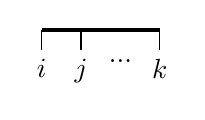
\begin{tikzpicture}
    \coordinate(origin1)at(0,.25);
    \draw[ultra thick]
        (origin1)--++(1.5,0)
    ;
    \draw
        (origin1)--++(0,-.25)
        node[anchor=north]{$i$}
        ++(.5,.25)--++(0,-.25)
        node[anchor=north]{$j$}
        ++(.5,0)node[anchor=north]{$...$}
        ++(.5,.25)--++(0,-.25)
        node[anchor=north]{$k$}
    ;
\end{tikzpicture}
}},
    \qquad
    \epsilon^{ij\cdots k}
    =
    \vcenter{\hbox{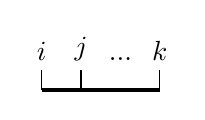
\begin{tikzpicture}
    \coordinate(origin1)at(0,.25);
    \coordinate(origin2)at(5,-.25);
    \draw[ultra thick]
        (origin2)--++(1.5,0)
    ;
    \draw
        (origin2)--++(0,.25)
        node[anchor=south]{$i$}
        ++(.5,-.25)--++(0,.25)
        node[anchor=south]{$j$}
        ++(.5,0)node[anchor=south]{$...$}
        ++(.5,-.25)--++(0,.25)
        node[anchor=south]{$k$}
    ;
\end{tikzpicture}
}}
\end{equation*}
Penroseの論文\cite{Penrose article}に合わせて階数が等しいLevi-Civitaテンソルの積は以下のように表すこともできる.
\footnote{Levi-Civitaテンソルの積というよりも「反対称化」の方が言葉は適しているだろう. $M^iB^j-B^iM^j$のような反対称テンソルを形成するときにはこの記法が有用である. }
\begin{equation*}
    \epsilon^{ij\cdots k}_{pq\cdots r}
    =
    \vcenter{\hbox{\begin{tikzpicture}
    \coordinate(origin)at(0,0);
    \draw[ultra thick]
        (origin)--++(1.5,0)
    ;
    \draw
        ($(origin)+(0,-.25)$)node[anchor=north]{$p$}
        --++(0,.5)node[anchor=south]{$i$}
        ++(.5,0)node[anchor=south]{$j$}
        --++(0,-.5)node[anchor=north]{$q$}
        ++(.5,0)node[anchor=north]{$\cdots$}
        ++(0,.5)node[anchor=south]{$\cdots$}
        ++(.5,0)node[anchor=south]{$k$}
        --++(0,-.5)
        node[anchor=north]{$r$}
        % ($(origin)+(2,0)$)node[anchor=west]{$\epsilon^{ij...k}\epsilon_{pq...r}$}
    ;
\end{tikzpicture}
}}
\end{equation*}
この正当性は
\begin{equation}
    \label{eq: Levi-Civita: product of Levi-Civita}
    \epsilon^{i_1\dots i_n}
    \epsilon_{j_1\dots j_n}
    =
    \epsilon^{i_1\dots i_n}_{1\dots n}
    \epsilon_{j_1\dots j_n}^{1\dots n}
    =
    \epsilon^{i_1\dots i_n}_{j_1\dots j_n}
\end{equation}
により保証される.


\subsubsection{計量テンソル}

計量テンソルは反変・共変に合わせてKroneckerの$\delta$を曲げたような格好になる.
\begin{equation*}
    g^{ij}
    =
    \vcenter{\hbox{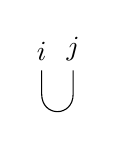
\begin{tikzpicture}
    \coordinate(origin1)at(0,0);
    \coordinate(origin2)at(3,0);
    \draw
    (origin1)node[anchor=south]{$i$}
    --++(0,-.3)
    .. controls ++(0,-.3) and ++(0,-.3) .. ++(.4,0)
    --++(0,.3)
    node[anchor=south]{$j$}
    ;
\end{tikzpicture}
}},
    \qquad
    g_{ij}
    =
    \vcenter{\hbox{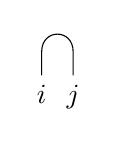
\begin{tikzpicture}
    \coordinate(origin1)at(0,0);
    \coordinate(origin2)at(3,0);
    \draw
    (origin2)node[anchor=north]{$i$}
    --++(0,.3)
    .. controls ++(0,.3) and ++(0,.3) .. ++(.4,0)
    --++(0,-.3)
    node[anchor=north]{$j$}
    ;
\end{tikzpicture}
}}
\end{equation*}


\subsection{Levi-Civitaテンソルの縮約公式}
\label{sec: levicivita: contraction}

\eqref{eq: Levi-Civita: product of Levi-Civita}を背景に, Euclid計量におけるLevi-Civitaテンソルの縮約はKroneckerの$\delta$の行列式を使って表されることが多い.
\begin{equation*}
    \epsilon^{ij\cdots k}\epsilon_{pq\cdots r}
    =
    \mqty|
        \delta^i_p & \delta^i_q & \cdots & \delta^i_r
        \\
        \delta^j_p & \delta^j_q & \cdots & \delta^j_r
        \\
        \vdots & \vdots & \ddots & \ddots
        \\
        \delta^k_p & \delta^k_q & \cdots & \delta^k_r
    |
\end{equation*}
一般次元, 一般計量での展開をPenroseのグラフ記法で表すと混乱を生じるので, はじめに3次元, 4次元のEuclid計量における縮約公式を取り上げる.


\subsubsection{3次元での縮約}

Kroneckerの$\delta$を使って縮約を愚直に書き出すと以下のようになる.
\begin{align*}
    \epsilon^{ijk}\epsilon_{pqr}
    &=
    \mqty|
        \delta^i_p & \delta^i_q & \delta^i_r
        \\
        \delta^j_p & \delta^j_q & \delta^j_r
        \\
        \delta^k_p & \delta^k_q & \delta^k_r
    |
    \\
    &=
    \delta^i_p\delta^j_q\delta^k_r
    -
    \delta^i_p\delta^j_r\delta^k_q
    +
    \delta^i_q\delta^j_r\delta^k_p
    -
    \delta^i_q\delta^j_p\delta^k_r
    +
    \delta^i_r\delta^j_p\delta^k_q
    -
    \delta^i_r\delta^j_q\delta^k_p
\end{align*}
\begin{equation*}
    \begin{tikzpicture}
    \coordinate(origin1)at(0,0);
    \node at(1.5,-.275)[anchor=center]{$=$};
    \coordinate(origin2)at(2,0);
    \node at(3.5,-.275)[anchor=center]{$-$};
    \coordinate(origin3)at(4,0);
    \node at(5.5,-.275)[anchor=center]{$+$};
    \coordinate(origin4)at(6,0);
    \node at(7.5,-.275)[anchor=center]{$-$};
    \coordinate(origin5)at(8,0);
    \node at(9.5,-.275)[anchor=center]{$+$};
    \coordinate(origin6)at(10,0);
    \node at(11.5,-.275)[anchor=center]{$-$};
    \coordinate(origin7)at(12,0);
    \draw[ultra thick]
        ($(origin1)+(0,-.25)$)--++(1,0)
    ;
    \draw
        (origin1)node[anchor=south]{$i$}
        --++(0,-.5)node[anchor=north]{$p$}
        ++(.5,.5)node[anchor=south]{$j$}
        --++(0,-.5)node[anchor=north]{$q$}
        ++(.5,.5)node[anchor=south]{$k$}
        --++(0,-.5)node[anchor=north]{$r$}
    ;
    \draw
        (origin2)node[anchor=south](i){$i$}
        ++(.5,0)node[anchor=south](j){$j$}
        ++(.5,0)node[anchor=south](k){$k$}
        ++(-1,-.55)node[anchor=north](p){$p$}
        ++(.5,0)node[anchor=north](q){$q$}
        ++(.5,0)node[anchor=north](r){$r$}
        (i.south)--(p.north)
        (j.south)--(q.north)
        (k.south)--(r.north)
    ;
    \draw
    (origin3)node[anchor=south](i){$i$}
    ++(.5,0)node[anchor=south](j){$j$}
    ++(.5,0)node[anchor=south](k){$k$}
    ++(-1,-.55)node[anchor=north](p){$p$}
    ++(.5,0)node[anchor=north](q){$q$}
    ++(.5,0)node[anchor=north](r){$r$}
    (i.south)--(p.north)
    (j.south)--(r.north)
    (k.south)--(q.north)
    ;
    \draw
    (origin4)node[anchor=south](i){$i$}
    ++(.5,0)node[anchor=south](j){$j$}
    ++(.5,0)node[anchor=south](k){$k$}
    ++(-1,-.55)node[anchor=north](p){$p$}
    ++(.5,0)node[anchor=north](q){$q$}
    ++(.5,0)node[anchor=north](r){$r$}
    (i.south)--(q.north)
    (j.south)--(r.north)
    (k.south)--(p.north)
    ;
    \draw
    (origin5)node[anchor=south](i){$i$}
    ++(.5,0)node[anchor=south](j){$j$}
    ++(.5,0)node[anchor=south](k){$k$}
    ++(-1,-.55)node[anchor=north](p){$p$}
    ++(.5,0)node[anchor=north](q){$q$}
    ++(.5,0)node[anchor=north](r){$r$}
    (i.south)--(q.north)
    (j.south)--(p.north)
    (k.south)--(r.north)
    ;
    \draw
    (origin6)node[anchor=south](i){$i$}
    ++(.5,0)node[anchor=south](j){$j$}
    ++(.5,0)node[anchor=south](k){$k$}
    ++(-1,-.55)node[anchor=north](p){$p$}
    ++(.5,0)node[anchor=north](q){$q$}
    ++(.5,0)node[anchor=north](r){$r$}
    (i.south)--(r.north)
    (j.south)--(p.north)
    (k.south)--(q.north)
    ;
    \draw
    (origin7)node[anchor=south](i){$i$}
    ++(.5,0)node[anchor=south](j){$j$}
    ++(.5,0)node[anchor=south](k){$k$}
    ++(-1,-.55)node[anchor=north](p){$p$}
    ++(.5,0)node[anchor=north](q){$q$}
    ++(.5,0)node[anchor=north](r){$r$}
    (i.south)--(r.north)
    (j.south)--(q.north)
    (k.south)--(p.north)
    ;
\end{tikzpicture}

\end{equation*}
上3本と下3本の端をつなぐ方法を全て列挙し, 置換に応じた符号を与えれば良い.

Levi-Civitaテンソルのグラフ記法が真価を発揮するのは一部の脚がつながっている場合だろう.

上下1組がつながっているときは\ref{sec: levi-civita contraction for vectors}で紹介した通りである.
縮約によってLevi-Civitaテンソルの次数が減ると捉えられる.
$i,j,k$及び$p,q,r$各組3つの中で互いに異なるものだけが値を持つことに注意しなければならない.
\begin{align*}
    \epsilon^{ijk}\epsilon_{pqk}
    &=
    \mqty|
        \delta^i_p & \delta^i_q & 0
        \\
        \delta^j_p & \delta^j_q & 0
        \\
        0 & 0 & 1
    |
    =
    \mqty|
        \delta^i_p & \delta^i_q
        \\
        \delta^j_p & \delta^j_q
    |
    \\
    &=\delta^i_p\delta^j_q-\delta^i_q\delta^j_p
\end{align*}
グラフ記法では縮約をとった部分を消去すれば良い.
\begin{equation*}
    \begin{tikzpicture}
    \coordinate(origin1)at(-.5,0);
    \node at(1.25,-.255)[anchor=center]{$=$};
    \coordinate(origin2)at(2,0);
    \node at(3.25,-.255)[anchor=center]{$=$};
    \coordinate(origin3)at(4,0);
    \node at(5.25,-.255)[anchor=center]{$-$};
    \coordinate(origin4)at(6,0);
    \draw[ultra thick]
        ($(origin1)-(0,.25)$)--++(1,0)
        ($(origin2)-(0,.25)$)--++(.5,0)
    ;
    \draw
        (origin1)node[anchor=south]{$i$}
        --++(0,-.5)node[anchor=north]{$p$}
        ++(.5,.5)node[anchor=south]{$j$}
        --++(0,-.5)node[anchor=north]{$q$}
        ++(.5,.5)node[anchor=south](k){}
        --++(0,-.5)node[anchor=north](r){}
        (k.south) .. controls ++(0,.1) and ++(0,.1) .. ++(.2,0)
        --++(0,-.5)
        .. controls ++(0,-.1) and ++(0,-.1) .. +(-.2,0)
    ;
    \draw
        (origin2)node[anchor=south]{$i$}
        --++(0,-.5)node[anchor=north]{$p$}
        ++(.5,.5)node[anchor=south]{$j$}
        --++(0,-.5)node[anchor=north]{$q$}
    ;
    \draw
        (origin3)node[anchor=south](i){$i$}
        ++(.5,0)node[anchor=south](j){$j$}
        ++(-.5,-.55)node[anchor=north](p){$p$}
        ++(.5,0)node[anchor=north](q){$q$}
        (i.south)--(p.north)
        (j.south)--(q.north)
    ;
    \draw
        (origin4)node[anchor=south](i){$i$}
        ++(.5,0)node[anchor=south](j){$j$}
        ++(-.5,-.55)node[anchor=north](p){$p$}
        ++(.5,0)node[anchor=north](q){$q$}
        (i.south)--(q.north)
        (j.south)--(p.north)
    ;
\end{tikzpicture}

\end{equation*}

2成分が縮約したときは, 縮約した2成分の並び方を考慮して$2!$をかけなければならない.
\begin{align*}
    \epsilon^{ijk}\epsilon_{pjk}
    =
    2!
    \mqty|
        \delta^i_p & 0 & 0
        \\
        0 & 1 & 0
        \\
        0 & 0 & 1
    |
    =2\delta^i_p
\end{align*}
\begin{equation*}
    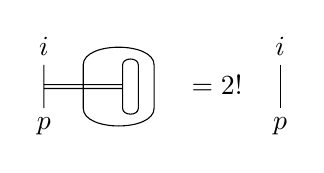
\begin{tikzpicture}
    \coordinate(origin1)at(-.5,0);
    \node at(1.7,-.255)[anchor=center]{$=2!$};
    \coordinate(origin2)at(2.5,0);
    \draw
    (origin1)node[anchor=south]{$i$}
    --++(0,-.55)node[anchor=north]{$p$}
    ++(.5,.55)node[anchor=south](j){}
    --++(0,-.55)node[anchor=north](q){}
    ++(.5,.55)node[anchor=south](k){}
    --++(0,-.55)node[anchor=north](r){}
    ++(0,.25)--++(-1,0)
    ++(0,.05)--++(1,0)
    (k.south) .. controls ++(0,.1) and ++(0,.1) .. ++(.2,0)
    --++(0,-.55)
    .. controls ++(0,-.1) and ++(0,-.1) .. (r.north)
    (j.south) .. controls ++(0,.3) and ++(0,.3) .. ++(.9,0)
    --++(0,-.55)
    .. controls ++(0,-.3) and ++(0,-.3) .. (q.north)
    ;
    \draw
    (origin2)node[anchor=south]{$i$}
    --++(0,-.55)node[anchor=north]{$p$}
    ;
\end{tikzpicture}

\end{equation*}
$2!$をかける理由はグラフ記法において直観的に理解できるだろう.
例として$i,j,k$及び$p,q,r$の3成分のうち, 上図のように$j,q$と$k,r$が縮約しているとする.
図の縮約を表す2本の線に対して, 内側に$j,q$を, 外側に$k,r$を当てる場合と, 内側に$k,r$外側に$j,q$を当てる場合の両方を足さなければならない.
この場合の数のために$2!$を要する.

同様にして3成分全てが縮約したときは$3!$をかけなければならない.
\begin{align*}
    \epsilon^{ijk}\epsilon_{ijk}
    =
    3!
    \mqty|
        1 & 0 & 0
        \\
        0 & 1 & 0
        \\
        0 & 0 & 1
    |
    =6
\end{align*}
\begin{equation*}
    \begin{tikzpicture}
    \coordinate(origin1)at(-.5,0);
    \node at(1.7,-.255)[anchor=center]{$=3!$};
    \coordinate(origin2)at(2.5,0);
    \draw[ultra thick]
        ($(origin1)-(0,.25)$)--++(1,0)
    ;
    \draw
        (origin1)node[anchor=south](i){}
        --++(0,-.5)node[anchor=north](p){}
        ++(.5,.5)node[anchor=south](j){}
        --++(0,-.5)node[anchor=north](q){}
        ++(.5,.5)node[anchor=south](k){}
        --++(0,-.5)node[anchor=north](r){}
        (k.south) .. controls ++(0,.1) and ++(0,.1) .. ++(.2,0)
        --++(0,-.5)
        .. controls ++(0,-.1) and ++(0,-.1) .. (r.north)
        (j.south) .. controls ++(0,.3) and ++(0,.3) .. ++(.9,0)
        --++(0,-.5)
        .. controls ++(0,-.3) and ++(0,-.3) .. (q.north)
        (i.south) .. controls ++(0,.5) and ++(0,.5) .. ++(1.6,0)
        --++(0,-.5)
        .. controls ++(0,-.5) and ++(0,-.5) .. (p.north)
    ;
\end{tikzpicture}

\end{equation*}
やはり$(i,p)$, $(j,q)$, $(k,r)$の組をそれぞれどの線に当てるかで$3!$通りあることから, 係数も直観的に理解できる.


\subsubsection{4次元での縮約}

以下引き続きEuclid計量で記述する.
Minkowski計量ではEuclidの4つの共変成分全てに計量テンソル
\begin{equation*}
    g_{ij}=
    \begin{cases}
        1 & i=j=0
        \\
        -1 & i=j\neq0
        \\
        0 & i\neq j
    \end{cases}
\end{equation*}
がかかり, 以下全ての結果に負号がつく.

Kroneckerの$\delta$を使って愚直に計算すると以下のようになる.
\begin{align*}
    \epsilon^{ijkl}\epsilon_{pqrs}
    =&
    \mqty|
        \delta^i_p & \delta^i_q & \delta^i_r & \delta^i_s
        \\
        \delta^j_p & \delta^j_q & \delta^j_r & \delta^j_s
        \\
        \delta^k_p & \delta^k_q & \delta^k_r & \delta^k_s
        \\
        \delta^l_p & \delta^l_q & \delta^l_r & \delta^l_s
    |
    \\
    =&
    \delta^i_p\delta^j_q\delta^k_r\delta^l_s
    -
    \delta^i_p\delta^j_q\delta^k_s\delta^l_r
    -
    \delta^i_p\delta^j_r\delta^k_q\delta^l_s
    +
    \delta^i_p\delta^j_r\delta^k_s\delta^l_q
    +
    \delta^i_p\delta^j_s\delta^k_q\delta^l_r
    -
    \delta^i_p\delta^j_s\delta^k_r\delta^l_q
    \\
    &
    -
    \delta^i_q\delta^j_p\delta^k_r\delta^l_s
    +
    \delta^i_q\delta^j_p\delta^k_s\delta^l_r
    +
    \delta^i_q\delta^j_r\delta^k_p\delta^l_s
    -
    \delta^i_q\delta^j_r\delta^k_s\delta^l_p
    -
    \delta^i_q\delta^j_s\delta^k_p\delta^l_r
    +
    \delta^i_q\delta^j_s\delta^k_r\delta^l_p
    \\
    &
    +
    \delta^i_r\delta^j_p\delta^k_q\delta^l_s
    -
    \delta^i_r\delta^j_p\delta^k_s\delta^l_q
    -
    \delta^i_r\delta^j_q\delta^k_p\delta^l_s
    +
    \delta^i_r\delta^j_q\delta^k_s\delta^l_p
    +
    \delta^i_r\delta^j_s\delta^k_p\delta^l_q
    -
    \delta^i_r\delta^j_s\delta^k_q\delta^l_p
    \\
    &-
    \delta^i_s\delta^j_p\delta^k_q\delta^l_r
    +
    \delta^i_s\delta^j_p\delta^k_r\delta^l_q
    +
    \delta^i_s\delta^j_q\delta^k_p\delta^l_r
    -
    \delta^i_s\delta^j_q\delta^k_r\delta^l_p
    -
    \delta^i_s\delta^j_r\delta^k_p\delta^l_q
    +
    \delta^i_s\delta^j_r\delta^k_q\delta^l_p
\end{align*}
これを図示してもやはり長大になることに変わりない.
\begin{equation*}
    \begin{tikzpicture}
    \coordinate(origin0)at(0,0);
    \coordinate(origin1)at(2.5,0);
    \coordinate(origin2)at(5,0);
    \coordinate(origin3)at(7.5,0);
    \coordinate(origin4)at(2.5,-2);
    \coordinate(origin5)at(5,-2);
    \coordinate(origin6)at(7.5,-2);
    \coordinate(origin7)at(2.5,-4);
    \coordinate(origin8)at(5,-4);
    \coordinate(origin9)at(7.5,-4);
    \coordinate(origin10)at(2.5,-6);
    \coordinate(origin11)at(5,-6);
    \coordinate(origin12)at(7.5,-6);
    \coordinate(origin13)at(2.5,-8);
    \coordinate(origin14)at(5,-8);
    \coordinate(origin15)at(7.5,-8);
    \coordinate(origin16)at(2.5,-10);
    \coordinate(origin17)at(5,-10);
    \coordinate(origin18)at(7.5,-10);
    \coordinate(origin19)at(2.5,-12);
    \coordinate(origin20)at(5,-12);
    \coordinate(origin21)at(7.5,-12);
    \coordinate(origin22)at(2.5,-14);
    \coordinate(origin23)at(5,-14);
    \coordinate(origin24)at(7.5,-14);
    \node at(2,-.255)[anchor=center]{$=$};
    \node at(4.5,-.255)[anchor=center]{$-$};
    \node at(7,-.255)[anchor=center]{$-$};
    \node at(2,-2.255)[anchor=center]{$+$};
    \node at(4.5,-2.255)[anchor=center]{$+$};
    \node at(7,-2.255)[anchor=center]{$-$};
    \node at(2,-4.255)[anchor=center]{$-$};
    \node at(4.5,-4.255)[anchor=center]{$+$};
    \node at(7,-4.255)[anchor=center]{$+$};
    \node at(2,-6.255)[anchor=center]{$-$};
    \node at(4.5,-6.255)[anchor=center]{$-$};
    \node at(7,-6.255)[anchor=center]{$+$};
    \node at(2,-8.255)[anchor=center]{$+$};
    \node at(4.5,-8.255)[anchor=center]{$-$};
    \node at(7,-8.255)[anchor=center]{$-$};
    \node at(2,-10.255)[anchor=center]{$+$};
    \node at(4.5,-10.255)[anchor=center]{$+$};
    \node at(7,-10.255)[anchor=center]{$-$};
    \node at(2,-12.255)[anchor=center]{$-$};
    \node at(4.5,-12.255)[anchor=center]{$+$};
    \node at(7,-12.255)[anchor=center]{$+$};
    \node at(2,-14.255)[anchor=center]{$-$};
    \node at(4.5,-14.255)[anchor=center]{$-$};
    \node at(7,-14.255)[anchor=center]{$+$};
    % LHS
    \draw[ultra thick]
        ($(origin0)+(0,-.25)$)--++(1.5,0)
    ;
    \draw
        (origin0)node[anchor=south](i){$i$}
        ++(.5,0)node[anchor=south](j){$j$}
        ++(.5,0)node[anchor=south](k){$k$}
        ++(.5,0)node[anchor=south](l){$l$}
        ++(-1.5,-.5)node[anchor=north](p){$p$}
        ++(.5,0)node[anchor=north](q){$q$}
        ++(.5,0)node[anchor=north](r){$r$}
        ++(.5,0)node[anchor=north](s){$s$}
        (i.south)--(p.north)
        (j.south)--(q.north)
        (k.south)--(r.north)
        (l.south)--(s.north)
    ;
    % RHS 1st
    \draw
    (origin1)node[anchor=south](i){$i$}
    ++(.5,0)node[anchor=south](j){$j$}
    ++(.5,0)node[anchor=south](k){$k$}
    ++(.5,0)node[anchor=south](l){$l$}
    ++(-1.5,-.55)node[anchor=north](p){$p$}
    ++(.5,0)node[anchor=north](q){$q$}
    ++(.5,0)node[anchor=north](r){$r$}
    ++(.5,0)node[anchor=north](s){$s$}
    (i.south)--(p.north)
    (j.south)--(q.north)
    (k.south)--(r.north)
    (l.south)--(s.north)
    ;
    \draw
    (origin2)node[anchor=south](i){$i$}
    ++(.5,0)node[anchor=south](j){$j$}
    ++(.5,0)node[anchor=south](k){$k$}
    ++(.5,0)node[anchor=south](l){$l$}
    ++(-1.5,-.55)node[anchor=north](p){$p$}
    ++(.5,0)node[anchor=north](q){$q$}
    ++(.5,0)node[anchor=north](r){$r$}
    ++(.5,0)node[anchor=north](s){$s$}
    (i.south)--(p.north)
    (j.south)--(q.north)
    (k.south)--(s.north)
    (l.south)--(r.north)
    ;
    \draw
    (origin3)node[anchor=south](i){$i$}
    ++(.5,0)node[anchor=south](j){$j$}
    ++(.5,0)node[anchor=south](k){$k$}
    ++(.5,0)node[anchor=south](l){$l$}
    ++(-1.5,-.55)node[anchor=north](p){$p$}
    ++(.5,0)node[anchor=north](q){$q$}
    ++(.5,0)node[anchor=north](r){$r$}
    ++(.5,0)node[anchor=north](s){$s$}
    (i.south)--(p.north)
    (j.south)--(r.north)
    (k.south)--(q.north)
    (l.south)--(s.north)
    ;
    % RHS 2nd
    \draw
    (origin4)node[anchor=south](i){$i$}
    ++(.5,0)node[anchor=south](j){$j$}
    ++(.5,0)node[anchor=south](k){$k$}
    ++(.5,0)node[anchor=south](l){$l$}
    ++(-1.5,-.55)node[anchor=north](p){$p$}
    ++(.5,0)node[anchor=north](q){$q$}
    ++(.5,0)node[anchor=north](r){$r$}
    ++(.5,0)node[anchor=north](s){$s$}
    (i.south)--(p.north)
    (j.south)--(r.north)
    (k.south)--(s.north)
    (l.south)--(q.north)
    ;
    \draw
    (origin5)node[anchor=south](i){$i$}
    ++(.5,0)node[anchor=south](j){$j$}
    ++(.5,0)node[anchor=south](k){$k$}
    ++(.5,0)node[anchor=south](l){$l$}
    ++(-1.5,-.55)node[anchor=north](p){$p$}
    ++(.5,0)node[anchor=north](q){$q$}
    ++(.5,0)node[anchor=north](r){$r$}
    ++(.5,0)node[anchor=north](s){$s$}
    (i.south)--(p.north)
    (j.south)--(s.north)
    (k.south)--(q.north)
    (l.south)--(r.north)
    ;
    \draw
    (origin6)node[anchor=south](i){$i$}
    ++(.5,0)node[anchor=south](j){$j$}
    ++(.5,0)node[anchor=south](k){$k$}
    ++(.5,0)node[anchor=south](l){$l$}
    ++(-1.5,-.55)node[anchor=north](p){$p$}
    ++(.5,0)node[anchor=north](q){$q$}
    ++(.5,0)node[anchor=north](r){$r$}
    ++(.5,0)node[anchor=north](s){$s$}
    (i.south)--(p.north)
    (j.south)--(s.north)
    (k.south)--(r.north)
    (l.south)--(q.north)
    ;
    % RHS 3rd
    \draw
    (origin7)node[anchor=south](i){$i$}
    ++(.5,0)node[anchor=south](j){$j$}
    ++(.5,0)node[anchor=south](k){$k$}
    ++(.5,0)node[anchor=south](l){$l$}
    ++(-1.5,-.55)node[anchor=north](p){$p$}
    ++(.5,0)node[anchor=north](q){$q$}
    ++(.5,0)node[anchor=north](r){$r$}
    ++(.5,0)node[anchor=north](s){$s$}
    (i.south)--(q.north)
    (j.south)--(p.north)
    (k.south)--(r.north)
    (l.south)--(s.north)
    ;
    \draw
    (origin8)node[anchor=south](i){$i$}
    ++(.5,0)node[anchor=south](j){$j$}
    ++(.5,0)node[anchor=south](k){$k$}
    ++(.5,0)node[anchor=south](l){$l$}
    ++(-1.5,-.55)node[anchor=north](p){$p$}
    ++(.5,0)node[anchor=north](q){$q$}
    ++(.5,0)node[anchor=north](r){$r$}
    ++(.5,0)node[anchor=north](s){$s$}
    (i.south)--(q.north)
    (j.south)--(p.north)
    (k.south)--(s.north)
    (l.south)--(r.north)
    ;
    \draw
    (origin9)node[anchor=south](i){$i$}
    ++(.5,0)node[anchor=south](j){$j$}
    ++(.5,0)node[anchor=south](k){$k$}
    ++(.5,0)node[anchor=south](l){$l$}
    ++(-1.5,-.55)node[anchor=north](p){$p$}
    ++(.5,0)node[anchor=north](q){$q$}
    ++(.5,0)node[anchor=north](r){$r$}
    ++(.5,0)node[anchor=north](s){$s$}
    (i.south)--(q.north)
    (j.south)--(r.north)
    (k.south)--(p.north)
    (l.south)--(s.north)
    ;
    % RHS 4th
    \draw
    (origin10)node[anchor=south](i){$i$}
    ++(.5,0)node[anchor=south](j){$j$}
    ++(.5,0)node[anchor=south](k){$k$}
    ++(.5,0)node[anchor=south](l){$l$}
    ++(-1.5,-.55)node[anchor=north](p){$p$}
    ++(.5,0)node[anchor=north](q){$q$}
    ++(.5,0)node[anchor=north](r){$r$}
    ++(.5,0)node[anchor=north](s){$s$}
    (i.south)--(q.north)
    (j.south)--(r.north)
    (k.south)--(s.north)
    (l.south)--(p.north)
    ;
    \draw
    (origin11)node[anchor=south](i){$i$}
    ++(.5,0)node[anchor=south](j){$j$}
    ++(.5,0)node[anchor=south](k){$k$}
    ++(.5,0)node[anchor=south](l){$l$}
    ++(-1.5,-.55)node[anchor=north](p){$p$}
    ++(.5,0)node[anchor=north](q){$q$}
    ++(.5,0)node[anchor=north](r){$r$}
    ++(.5,0)node[anchor=north](s){$s$}
    (i.south)--(q.north)
    (j.south)--(s.north)
    (k.south)--(p.north)
    (l.south)--(r.north)
    ;
    \draw
    (origin12)node[anchor=south](i){$i$}
    ++(.5,0)node[anchor=south](j){$j$}
    ++(.5,0)node[anchor=south](k){$k$}
    ++(.5,0)node[anchor=south](l){$l$}
    ++(-1.5,-.55)node[anchor=north](p){$p$}
    ++(.5,0)node[anchor=north](q){$q$}
    ++(.5,0)node[anchor=north](r){$r$}
    ++(.5,0)node[anchor=north](s){$s$}
    (i.south)--(q.north)
    (j.south)--(s.north)
    (k.south)--(r.north)
    (l.south)--(p.north)
    ;
    % RHS 5th
    \draw
    (origin13)node[anchor=south](i){$i$}
    ++(.5,0)node[anchor=south](j){$j$}
    ++(.5,0)node[anchor=south](k){$k$}
    ++(.5,0)node[anchor=south](l){$l$}
    ++(-1.5,-.55)node[anchor=north](p){$p$}
    ++(.5,0)node[anchor=north](q){$q$}
    ++(.5,0)node[anchor=north](r){$r$}
    ++(.5,0)node[anchor=north](s){$s$}
    (i.south)--(r.north)
    (j.south)--(p.north)
    (k.south)--(q.north)
    (l.south)--(s.north)
    ;
    \draw
    (origin14)node[anchor=south](i){$i$}
    ++(.5,0)node[anchor=south](j){$j$}
    ++(.5,0)node[anchor=south](k){$k$}
    ++(.5,0)node[anchor=south](l){$l$}
    ++(-1.5,-.55)node[anchor=north](p){$p$}
    ++(.5,0)node[anchor=north](q){$q$}
    ++(.5,0)node[anchor=north](r){$r$}
    ++(.5,0)node[anchor=north](s){$s$}
    (i.south)--(r.north)
    (j.south)--(p.north)
    (k.south)--(s.north)
    (l.south)--(q.north)
    ;
    \draw
    (origin15)node[anchor=south](i){$i$}
    ++(.5,0)node[anchor=south](j){$j$}
    ++(.5,0)node[anchor=south](k){$k$}
    ++(.5,0)node[anchor=south](l){$l$}
    ++(-1.5,-.55)node[anchor=north](p){$p$}
    ++(.5,0)node[anchor=north](q){$q$}
    ++(.5,0)node[anchor=north](r){$r$}
    ++(.5,0)node[anchor=north](s){$s$}
    (i.south)--(r.north)
    (j.south)--(q.north)
    (k.south)--(p.north)
    (l.south)--(s.north)
    ;
    % RHS 6th
    \draw
    (origin16)node[anchor=south](i){$i$}
    ++(.5,0)node[anchor=south](j){$j$}
    ++(.5,0)node[anchor=south](k){$k$}
    ++(.5,0)node[anchor=south](l){$l$}
    ++(-1.5,-.55)node[anchor=north](p){$p$}
    ++(.5,0)node[anchor=north](q){$q$}
    ++(.5,0)node[anchor=north](r){$r$}
    ++(.5,0)node[anchor=north](s){$s$}
    (i.south)--(r.north)
    (j.south)--(q.north)
    (k.south)--(s.north)
    (l.south)--(p.north)
    ;
    \draw
    (origin17)node[anchor=south](i){$i$}
    ++(.5,0)node[anchor=south](j){$j$}
    ++(.5,0)node[anchor=south](k){$k$}
    ++(.5,0)node[anchor=south](l){$l$}
    ++(-1.5,-.55)node[anchor=north](p){$p$}
    ++(.5,0)node[anchor=north](q){$q$}
    ++(.5,0)node[anchor=north](r){$r$}
    ++(.5,0)node[anchor=north](s){$s$}
    (i.south)--(r.north)
    (j.south)--(s.north)
    (k.south)--(p.north)
    (l.south)--(q.north)
    ;
    \draw
    (origin18)node[anchor=south](i){$i$}
    ++(.5,0)node[anchor=south](j){$j$}
    ++(.5,0)node[anchor=south](k){$k$}
    ++(.5,0)node[anchor=south](l){$l$}
    ++(-1.5,-.55)node[anchor=north](p){$p$}
    ++(.5,0)node[anchor=north](q){$q$}
    ++(.5,0)node[anchor=north](r){$r$}
    ++(.5,0)node[anchor=north](s){$s$}
    (i.south)--(r.north)
    (j.south)--(s.north)
    (k.south)--(q.north)
    (l.south)--(p.north)
    ;
    % RHS 7th
    \draw
    (origin19)node[anchor=south](i){$i$}
    ++(.5,0)node[anchor=south](j){$j$}
    ++(.5,0)node[anchor=south](k){$k$}
    ++(.5,0)node[anchor=south](l){$l$}
    ++(-1.5,-.55)node[anchor=north](p){$p$}
    ++(.5,0)node[anchor=north](q){$q$}
    ++(.5,0)node[anchor=north](r){$r$}
    ++(.5,0)node[anchor=north](s){$s$}
    (i.south)--(s.north)
    (j.south)--(p.north)
    (k.south)--(q.north)
    (l.south)--(r.north)
    ;
    \draw
    (origin20)node[anchor=south](i){$i$}
    ++(.5,0)node[anchor=south](j){$j$}
    ++(.5,0)node[anchor=south](k){$k$}
    ++(.5,0)node[anchor=south](l){$l$}
    ++(-1.5,-.55)node[anchor=north](p){$p$}
    ++(.5,0)node[anchor=north](q){$q$}
    ++(.5,0)node[anchor=north](r){$r$}
    ++(.5,0)node[anchor=north](s){$s$}
    (i.south)--(s.north)
    (j.south)--(p.north)
    (k.south)--(r.north)
    (l.south)--(q.north)
    ;
    \draw
    (origin21)node[anchor=south](i){$i$}
    ++(.5,0)node[anchor=south](j){$j$}
    ++(.5,0)node[anchor=south](k){$k$}
    ++(.5,0)node[anchor=south](l){$l$}
    ++(-1.5,-.55)node[anchor=north](p){$p$}
    ++(.5,0)node[anchor=north](q){$q$}
    ++(.5,0)node[anchor=north](r){$r$}
    ++(.5,0)node[anchor=north](s){$s$}
    (i.south)--(s.north)
    (j.south)--(q.north)
    (k.south)--(p.north)
    (l.south)--(r.north)
    ;
    % RHS 8th
    \draw
    (origin22)node[anchor=south](i){$i$}
    ++(.5,0)node[anchor=south](j){$j$}
    ++(.5,0)node[anchor=south](k){$k$}
    ++(.5,0)node[anchor=south](l){$l$}
    ++(-1.5,-.55)node[anchor=north](p){$p$}
    ++(.5,0)node[anchor=north](q){$q$}
    ++(.5,0)node[anchor=north](r){$r$}
    ++(.5,0)node[anchor=north](s){$s$}
    (i.south)--(s.north)
    (j.south)--(q.north)
    (k.south)--(r.north)
    (l.south)--(p.north)
    ;
    \draw
    (origin23)node[anchor=south](i){$i$}
    ++(.5,0)node[anchor=south](j){$j$}
    ++(.5,0)node[anchor=south](k){$k$}
    ++(.5,0)node[anchor=south](l){$l$}
    ++(-1.5,-.55)node[anchor=north](p){$p$}
    ++(.5,0)node[anchor=north](q){$q$}
    ++(.5,0)node[anchor=north](r){$r$}
    ++(.5,0)node[anchor=north](s){$s$}
    (i.south)--(s.north)
    (j.south)--(r.north)
    (k.south)--(p.north)
    (l.south)--(q.north)
    ;
    \draw
    (origin24)node[anchor=south](i){$i$}
    ++(.5,0)node[anchor=south](j){$j$}
    ++(.5,0)node[anchor=south](k){$k$}
    ++(.5,0)node[anchor=south](l){$l$}
    ++(-1.5,-.55)node[anchor=north](p){$p$}
    ++(.5,0)node[anchor=north](q){$q$}
    ++(.5,0)node[anchor=north](r){$r$}
    ++(.5,0)node[anchor=north](s){$s$}
    (i.south)--(s.north)
    (j.south)--(r.north)
    (k.south)--(q.north)
    (l.south)--(p.north)
    ;
\end{tikzpicture}

\end{equation*}

縮約を受けると次元が下がるのも同じである.
3次元の場合と同様, 縮約をとった部分は消去する.
\begin{align*}
    \epsilon^{ijkl}\epsilon_{pqrl}
    &=
    \mqty|
        \delta^i_p & \delta^i_q & \delta^i_r & 0
        \\
        \delta^j_p & \delta^j_q & \delta^j_r & 0
        \\
        \delta^k_p & \delta^k_q & \delta^k_r & 0
        \\
        0 & 0 & 0 & 1
    |
    =
    \mqty|
    \delta^i_p & \delta^i_q & \delta^i_r
    \\
    \delta^j_p & \delta^j_q & \delta^j_r
    \\
    \delta^k_p & \delta^k_q & \delta^k_r
    |;
    \qquad
    \vcenter{\hbox{\begin{tikzpicture}
    \coordinate(origin0)at(0,0);
    \coordinate(origin1)at(3,0);
    \node at(2.3,-.255)[anchor=center]{$=$};
    % LHS
    \draw
    (origin0)node[anchor=south](i){$i$}
    ++(.5,0)node[anchor=south](j){$j$}
    ++(.5,0)node[anchor=south](k){$k$}
    ++(.5,0)node[anchor=south](l){}
    ++(-1.5,-.55)node[anchor=north](p){$p$}
    ++(.5,0)node[anchor=north](q){$q$}
    ++(.5,0)node[anchor=north](r){$r$}
    ++(.5,0)node[anchor=north](s){}
    (i.south)--(p.north)
    (j.south)--(q.north)
    (k.south)--(r.north)
    (l.south)--(s.north)
    ($(origin0)+(0,-.25)$)--++(1.5,0)
    ++(0,-.05)--++(-1.5,0)
    (l.south)..controls ++(0,.5) and ++(.0,.5) .. ++(.2,0)
    --++(0,-.55)
    .. controls ++(0,-.5) and ++(0,-.5) .. ++(-.2,0)
    ;
    % RHS
    \draw
    (origin1)node[anchor=south](i){$i$}
    --++(0,-.55)node[anchor=north](p){$p$}
    ++(.5,.55)node[anchor=south](j){$j$}
    --++(0,-.55)node[anchor=north](q){$q$}
    ++(.5,.55)node[anchor=south](k){$k$}
    --++(0,-.55)node[anchor=north](r){$r$}
    ++(0,.25)--++(-1,0)
    ++(0,.05)--++(1,0)
    ;
\end{tikzpicture}
}}
\end{align*}
複数の成分が縮約されれば$2!,3!,4!$をかける.
\begin{align*}
    \epsilon^{ijkl}\epsilon_{pqkl}
    &=
    2!
    \mqty|
        \delta^i_p & \delta^i_q & 0 & 0
        \\
        \delta^j_p & \delta^j_q & 0 & 0
        \\
        0 & 0 & 1 & 0
        \\
        0 & 0 & 0 & 1
    |
    % \\
    % &
    =
    2!
    \mqty|
        \delta^i_p & \delta^i_q
        \\
        \delta^j_p & \delta^j_q
    |;
    \qquad
    \vcenter{\hbox{\begin{tikzpicture}
    \coordinate(origin0)at(0,0);
    \coordinate(origin1)at(3,0);
    \node at(2.35,-.255)[anchor=center]{$=2!$};
    % LHS
    \draw[ultra thick]
        ($(origin0)+(0,-.25)$)--++(1.5,0)
    ;
    \draw
    (origin0)node[anchor=south](i){$i$}
    ++(.5,0)node[anchor=south](j){$j$}
    ++(.5,0)node[anchor=south](k){}
    ++(.5,0)node[anchor=south](l){}
    ++(-1.5,-.5)node[anchor=north](p){$p$}
    ++(.5,0)node[anchor=north](q){$q$}
    ++(.5,0)node[anchor=north](r){}
    ++(.5,0)node[anchor=north](s){}
    (i.south)--(p.north)
    (j.south)--(q.north)
    (k.south)--(r.north)
    (l.south)--(s.north)
    (l.south)..controls ++(0,.5) and ++(.0,.5) .. ++(.2,0)
    --++(0,-.5)
    .. controls ++(0,-.5) and ++(0,-.5) .. ++(-.2,0)
    (k.south) .. controls ++(0,.7) and ++(0,.7) .. ++(.9,0)
    --++(0,-.5)
    .. controls ++(0,-.7) and ++(0,-.7) .. ++(-.9,0)
    ;
    % RHS
    \draw[ultra thick]
        ($(origin1)-(0,.25)$)--++(.5,0)
    ;
    \draw
    (origin1)node[anchor=south](i){$i$}
    --++(0,-.5)node[anchor=north](p){$p$}
    ++(.5,.5)node[anchor=south](j){$j$}
    --++(0,-.5)node[anchor=north](q){$q$}
    ;
\end{tikzpicture}
}}
\end{align*}
\begin{align*}
    \epsilon^{ijkl}\epsilon_{pjkl}
    &=
    3!
    \mqty|
        \delta^i_p & 0 & 0 & 0
        \\
        0 & 1 & 0 & 0
        \\
        0 & 0 & 1 & 0
        \\
        0 & 0 & 0 & 1
    |
    % \\
    % &
    =
    3!
    \delta^i_p;
    \qquad
    \vcenter{\hbox{\begin{tikzpicture}
    \coordinate(origin0)at(0,0);
    \coordinate(origin1)at(3.5,0);
    \node at(2.7,-.255)[anchor=center]{$=3!$};
    % LHS
    \draw
    (origin0)node[anchor=south](i){$i$}
    ++(.5,0)node[anchor=south](j){}
    ++(.5,0)node[anchor=south](k){}
    ++(.5,0)node[anchor=south](l){}
    ++(-1.5,-.55)node[anchor=north](p){$p$}
    ++(.5,0)node[anchor=north](q){}
    ++(.5,0)node[anchor=north](r){}
    ++(.5,0)node[anchor=north](s){}
    (i.south)--(p.north)
    (j.south)--(q.north)
    (k.south)--(r.north)
    (l.south)--(s.north)
    ($(origin0)+(0,-.25)$)--++(1.5,0)
    ++(0,-.05)--++(-1.5,0)
    (l.south)..controls ++(0,.5) and ++(.0,.5) .. ++(.2,0)
    --++(0,-.55)
    .. controls ++(0,-.5) and ++(0,-.5) .. ++(-.2,0)
    (k.south) .. controls ++(0,.7) and ++(0,.7) .. ++(.9,0)
    --++(0,-.55)
    .. controls ++(0,-.7) and ++(0,-.7) .. ++(-.9,0)
    (j.south) .. controls ++(0,.9) and ++(0,.9) .. ++(1.6,0)
    --++(0,-.55)
    .. controls ++(0,-.9) and ++(0,-.9) .. ++(-1.6,0)
    ;
    % RHS
    \draw
    (origin1)node[anchor=south](i){$i$}
    --++(0,-.55)node[anchor=north](p){$p$}
    ;
\end{tikzpicture}
}}
\end{align*}
\begin{align*}
    \epsilon^{ijkl}\epsilon_{ijkl}
    &=
    % 4!
    % \mqty|
    %     1 & 0 & 0 & 0
    %     \\
    %     0 & 1 & 0 & 0
    %     \\
    %     0 & 0 & 1 & 0
    %     \\
    %     0 & 0 & 0 & 1
    % |
    % \\
    % &=
    4!;
    \qquad
    \vcenter{\hbox{\begin{tikzpicture}
    \coordinate(origin0)at(0,0);
    \coordinate(origin1)at(3.5,0);
    \node at(2.7,-.255)[anchor=center]{$=4!$};
    % LHS
    \draw
    (origin0)node[anchor=south](i){}
    ++(.5,0)node[anchor=south](j){}
    ++(.5,0)node[anchor=south](k){}
    ++(.5,0)node[anchor=south](l){}
    ++(-1.5,-.55)node[anchor=north](p){}
    ++(.5,0)node[anchor=north](q){}
    ++(.5,0)node[anchor=north](r){}
    ++(.5,0)node[anchor=north](s){}
    (i.south)--(p.north)
    (j.south)--(q.north)
    (k.south)--(r.north)
    (l.south)--(s.north)
    ($(origin0)+(0,-.25)$)--++(1.5,0)
    ++(0,-.05)--++(-1.5,0)
    (l.south)..controls ++(0,.5) and ++(.0,.5) .. ++(.2,0)
    --++(0,-.55)
    .. controls ++(0,-.5) and ++(0,-.5) .. ++(-.2,0)
    (k.south) .. controls ++(0,.7) and ++(0,.7) .. ++(.9,0)
    --++(0,-.55)
    .. controls ++(0,-.7) and ++(0,-.7) .. ++(-.9,0)
    (j.south) .. controls ++(0,.9) and ++(0,.9) .. ++(1.6,0)
    --++(0,-.55)
    .. controls ++(0,-.9) and ++(0,-.9) .. ++(-1.6,0)
    (i.south) .. controls ++(0,1.1) and ++(0,1.1) .. ++(2.3,0)
    --++(0,-.55)
    .. controls ++(0,-1.1) and ++(0,-1.1) .. ++(-2.3,0)
    ;
\end{tikzpicture}
}}
\end{align*}


\subsubsection{一般次元・計量での縮約}
\label{sec: levicivita: general dim and metric contraction}

ここまでの議論を踏まえて一般次元の, 計量が入った多様体における縮約公式を確認する.
Minkovski計量に代表されるように, 計量は必ずしも正定値とは限らない.

脚が$k+n$本のLevi-Civitaテンソルと$l+n$本のものとで, $n$本の脚を縮約している場合は,
\begin{equation}
    \label{eq: levicivita: contraction of levi-civita in general dim}
    \vcenter{\hbox{
        \begin{tikzpicture}
            \tikzmath{
                \yu=0;
                \yd=-2;
            }
            \draw[ultra thick]
                (0,\yu)--(2.5,\yu)
                (.7,\yd)--(2.5,\yd)
            ;
            \draw
                % open lines
                (.1,\yu)--++(0,-.25)
                node[anchor=north](mu1){$\mu_1$}
                (.8,\yu)--++(0,-.25)
                node[anchor=north](muk){$\mu_k$}
                (1.5,\yu)--++(0,-.25)
                node[anchor=north](mul){$\mu_l$}
                (.8,\yd)--++(0,+.25)
                node[anchor=south](nuk){$\nu_k$}
                (1.5,\yd)--++(0,+.25)
                node[anchor=south](nul){$\nu_l$}
                % connected lines
                (1.8,\yu)--(1.8,\yd)
                (2.4,\yu)--(2.4,\yd)
                % dots
                ($(mu1.north)!.5!(muk.north)$)node[anchor=center]{$\cdots$}
                ($(muk.north)!.5!(mul.north)$)node[anchor=center]{$\cdots$}
                ($(nuk.south)!.5!(nul.south)$)node[anchor=center]{$\cdots$}
                (2.1,{(\yu+\yd)/2})node[anchor=center]{$\cdots$}
            ;
            \draw[<->, dashed, >=Stealth](1.7,.2)--(2.5,.2);
            \node at(2.1,.2)[anchor=south]{$n$};
        \end{tikzpicture}
    }}
    =
    n!
    \vcenter{\hbox{
        \begin{tikzpicture}
            \draw[ultra thick](0,0)--(1.6,0);
            \draw
                (.1,0)--++(0,-.25)
                node[anchor=north](mu1){$\mu_1$}
                (.8,0)--++(0,-.25)
                node[anchor=north](muk){$\mu_k$}
                (.8,0)--++(0,.25)
                node[anchor=south](nuk){$\nu_k$}
                (1.5,0)--++(0,-.25)
                node[anchor=north](mul){$\mu_l$}
                (1.5,0)--++(0,.25)
                node[anchor=south](nul){$\nu_l$}
                ($(mu1.north)!.5!(muk.north)$)node[anchor=center]{$\cdots$}
                ($(mul.north)!.5!(muk.north)$)node[anchor=center]{$\cdots$}
                ($(nul.south)!.5!(nuk.south)$)node[anchor=center]{$\cdots$}
            ;
        \end{tikzpicture}
    }}
\end{equation}
となる.
合計$n$本の縮約があるとき, 縮約されている脚の順列$n!$の数だけ全く同じ値を返すことから理解される.
残った脚の数は同じでなくても構わない.
ただし, 残った脚がどの添字を取りうるかに注意しなければならない.
例えば,
\begin{equation*}
    \vcenter{\hbox{
        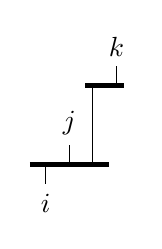
\begin{tikzpicture}
            \draw[ultra thick](0,0)--++(1,0);
            \draw[ultra thick](.7,1)--++(.5,0);
            \draw
                (.8,0)--++(0,1)
                (.5,0)--++(0,.25)node[anchor=south]{$j$}
                (.2,0)--++(0,-.25)node[anchor=north]{$i$}
                (1.1,1)--++(0,.25)node[anchor=south]{$k$}
            ;
        \end{tikzpicture}
    }}
    \neq
    \vcenter{\hbox{
        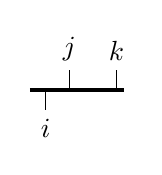
\begin{tikzpicture}
            \draw[ultra thick](0,0)--++(1.2,0);
            \draw
                (.5,0)--++(0,.25)node[anchor=south]{$j$}
                (.2,0)--++(0,-.25)node[anchor=north]{$i$}
                (1.1,0)--++(0,.25)node[anchor=south]{$k$}
            ;
        \end{tikzpicture}
    }}
\end{equation*}
である.
実際には$i\neq j=k$の場合と$i=k\neq j$の場合が残る.
また, 反変と共変を明確に区別するため, これまでのように安易に太線1本にまとめることはできない.

このような問題を背景に, Levi-Civitaテンソルを再定義したい.
% まずはRiemann多様体($g=\det(g_{\mu\nu})>0$)の場合を考える.
% Euclid計量$g^{(0)}$におけるLevi-Civitaテンソルを
% \begin{equation*}
%     \varepsilon_{\mu_1\cdots\mu_n}^{(0)}
%     =
%     \det\mqty(
%         \delta_{\mu_1}^1 & \cdots & \delta_{\mu_1}^n
%         \\
%         \vdots & \ddots & \vdots
%         \\
%         \delta_{\mu_n}^1 & \cdots & \delta_{\mu_n}^n
%     )
% \end{equation*}
% で与え, 一般座標変換$x^{(0)}\mapsto x$を考えると,
% \begin{equation*}
%     \varepsilon_{\mu_1\cdots\mu_n}
%     =
%     \pdv{x^{(0)\nu_1}}{x^{\mu_1}}
%     \cdots
%     \pdv{x^{(0)\nu_n}}{x^{\mu_n}}
%     \varepsilon_{\nu_1\cdots\nu_n}^{(0)}
%     =
%     \pdv{(x^{(0)1},\cdots,x^{(0)n})}{x^1,\cdots,x^n}
%     \varepsilon_{\nu_1\cdots\nu_n}^{(0)}
%     =
%     J
%     \varepsilon_{\nu_1\cdots\nu_n}^{(0)}
% \end{equation*}
% と, Jacobianが現れる.
% 計量テンソルの変換式
% \begin{equation*}
%     g_{\mu\nu}
%     =
%     \pdv{x^{(0)\rho}}{x^\mu}
%     g^{(0)}_{\rho\sigma}
%     \pdv{x^{(0)\sigma}}{x^\nu}
% \end{equation*}
% の両辺で行列式を考えると,
% \begin{equation*}
%     g
%     =
%     J^2
% \end{equation*}
% となる.
% 一方, 擬Riemann多様体($g<0$)はEuclid計量から線素$\dd{s}$を常に不変にする変換を与えることができない.
% Minkovski計量からなら問題なく変換可能である.
% 上記の議論をそのまま追うことで
% \begin{equation*}
%     g=-J^2
% \end{equation*}
% が得られる.
% 以上より
% \begin{equation*}
%     J=\sqrt{|g|}
% \end{equation*}
% なので, Levi-Civitaテンソルは
% \begin{equation*}
%     \varepsilon_{\mu_1\cdots\mu_n}
%     =
%     \sqrt{|g|}\varepsilon_{\mu_1\cdots\mu_n}^{(0)}
% \end{equation*}
% と定義するのが妥当であろう.
まず共変Levi-Civitaテンソルを
\begin{equation*}
    \varepsilon_{\mu_1\cdots\mu_k}
    =
    \det\mqty(
        \delta_{\mu_1}^1 & \cdots & \delta_{\mu_1}^k
        \\
        \vdots & \ddots & \vdots
        \\
        \delta_{\mu_k}^1 & \cdots & \delta_{\mu_k}^k
    )
\end{equation*}
で与える.
\footnote{
    この定義はいささか恣意的であることを認めなければならない.
    特にEuclid計量, Minkovski計量などLevi-Civitaテンソルの具体形がわかる計量からの一般座標変換$x\to x'$が与えられるときは, 既知のLevi-Civitaテンソル$\varepsilon^{(0)}_{\mu_1\cdots\mu_k}$の座標変換
    \begin{equation*}
        \varepsilon_{\mu_1\cdots\mu_k}
        =
        \pdv{x^{\nu_1}}{x'^{\mu_1}}
        \cdots
        \pdv{x^{\nu_k}}{x'^{\mu_k}}
        \varepsilon^{(0)}_{\nu_1\cdots\nu_k}
    \end{equation*}
    を計算するべきである.
    $k$が空間(多様体)の次元$d$に等しいときは変換の係数がJacobianになって
    \begin{equation*}
        \varepsilon_{\mu_1\cdots\mu_d}
        =
        \sqrt{|g|}
        \varepsilon^{(0)}_{\mu_1\cdots\mu_d}
    \end{equation*}
    を得る.
}
反変テンソルは計量テンソルによって
\begin{equation*}
    \varepsilon^{\mu_1\cdots\mu_k}
    =
    g^{\mu_1\nu_1}
    \cdots
    g^{\mu_k\nu_k}
    \varepsilon_{\nu_1\cdots\nu_k}
\end{equation*}
とする.
これを踏まえて
\begin{equation*}
    \vcenter{\hbox{
        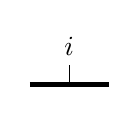
\begin{tikzpicture}
            \draw[ultra thick](0,0)--++(1,0);
            \draw(0.5,0)--++(0,.25)node[anchor=south]{$i$};
        \end{tikzpicture}
    }}
    =
    \vcenter{\hbox{
        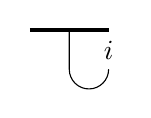
\begin{tikzpicture}
            \draw[ultra thick](0,0)--++(1,0);
            \draw(0.5,0)--++(0,-.5)arc(-180:0:.25)
            node[anchor=south]{$i$};
        \end{tikzpicture}
    }}
\end{equation*}
とできるので, 先ほどの例は
\begin{equation*}
    \vcenter{\hbox{
        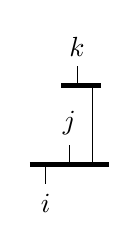
\begin{tikzpicture}
            \draw[ultra thick](0,0)--++(1,0);
            \draw[ultra thick](.4,1)--++(.5,0);
            \draw
                (.8,0)--++(0,1)
                (.5,0)--++(0,.25)node[anchor=south]{$j$}
                (.2,0)--++(0,-.25)node[anchor=north]{$i$}
                (.6,1)--++(0,.25)node[anchor=south]{$k$}
            ;
        \end{tikzpicture}
    }}
    =
    \vcenter{\hbox{
        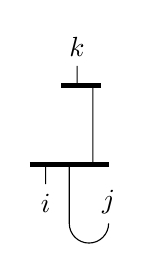
\begin{tikzpicture}
            \draw[ultra thick](0,0)--++(1,0);
            \draw[ultra thick](.4,1)--++(.5,0);
            \draw
                (.8,0)--++(0,1)
                (.5,0)--++(0,-.75)arc(-180:0:.25)node[anchor=south]{$j$}
                (.2,0)--++(0,-.25)node[anchor=north]{$i$}
                (.6,1)--++(0,.25)node[anchor=south]{$k$}
            ;
        \end{tikzpicture}
    }}
    =
    \vcenter{\hbox{
        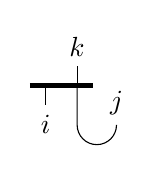
\begin{tikzpicture}
            \draw[ultra thick](0,0)--++(.8,0);
            \draw(.2,0)--++(0,-.25)node[anchor=north]{$i$};
            \draw(.6,0)--++(0,.25)node[anchor=south]{$k$};
            \draw(.6,0)--++(0,-.5)arc(-180:0:.25)node[anchor=south]{$j$};
        \end{tikzpicture}
    }}
\end{equation*}
と変形できる.

特に, 空間(多様体)の次元が$d$のとき,
\begin{equation}
    \label{eq: levicivita: covar-contravar change of d-component Levi-Civita}
    \varepsilon^{\mu_1\cdots\mu_d}
    =
    g^{\mu_1\nu_1}
    \cdots
    g^{\mu_d\nu_d}
    \varepsilon_{\nu_1\cdots\nu_d}
    =
    g^{-1}
    \varepsilon_{\mu_1\cdots\mu_d}
\end{equation}
である.
例えば
\begin{equation*}
    \vcenter{\hbox{
        \begin{tikzpicture}
            \coordinate(origin)at(0,0);
            \draw($(origin)+(0,.25)$)rectangle++(1.5,.4);
            \draw[ultra thick]($(origin)+(0,1)$)--++(3,0);
            \draw[ultra thick]($(origin)+(0,2)$)--++(3.2,0);
            \draw
                ($(origin)+(.1,.25)$)--++(0,-.5)node[anchor=north](mu1){}
                ++(.4,.5)--++(0,-.5)node[anchor=north](mu2){}
                ++(.5,0)node[anchor=center](cdots){$\cdots$}
                ($(origin)+(1.4,.25)$)--++(0,-.5)node[anchor=north](muk){}
                (mu1.north)
                arc(-180:0:.1)node[anchor=north](mu1up){}
                (mu2.north)
                arc(-180:0:.1)node[anchor=north](mu2up){}
                (muk.north)
                arc(-180:0:.1)node[anchor=north](mu3up){}
                ($(origin)+(2,1.)$)--++(0,-1.25)node[anchor=north](muk1){}
                ++(.5,.5)node[anchor=center]{$\cdots$}
                ($(origin)+(2.9,1.)$)--++(0,-1.25)node[anchor=north](mun){}
                (muk1.north)arc(-180:0:.1)node[anchor=north](muk1up){}
                (mun.north)arc(-180:0:.1)node[anchor=north](munup){}
                ($(origin)+(.2,2.)$)--++(0,-.5)
                node[anchor=north]{$\mu_1$}
                ++(.4,.5)--++(0,-.5)
                node[anchor=north]{$\mu_2$}
                ++(.5,.2)node[anchor=center]{$\cdots$}
                ($(origin)+(1.5,2)$)--++(0,-.5)
                node[anchor=north]{$\mu_k$}
            ;
            \draw[preaction={draw,white,line width=3pt}]
                (mu1up.north)--++(0,1.2)
                (mu2up.north)--++(0,1.2)
                (mu3up.north)--++(0,1.2)
                (muk1up.north)--++(0,2.2)
                (munup.north)--++(0,2.2)
            ;
            \draw[<->, >=Stealth, dashed]($(origin)+(0,-1.)$)--++(3.2,0);
            \node at(1.6,-1.)[anchor=north]{$d$};
            \draw[<->, >=Stealth, dashed]($(origin)+(0,-.5)$)--++(1.5,0);
            \node at(.8,-.5)[anchor=north]{$k$};
        \end{tikzpicture}
    }}
    =
    g^{-1}
    \vcenter{\hbox{
        \begin{tikzpicture}
            \coordinate(origin)at(0,0);
            \draw($(origin)+(0,.25)$)rectangle++(1.5,.4);
            \draw[ultra thick]($(origin)+(0,-.25)$)--++(3,0);
            \draw[ultra thick]($(origin)+(0,-.75)$)--++(3.,0);
            \draw
                ($(origin)+(.1,.25)$)--++(0,-.5)node[anchor=north](mu1){}
                ++(.4,.5)--++(0,-.5)node[anchor=north](mu2){}
                ++(.5,0)node[anchor=center](cdots){$\cdots$}
                ($(origin)+(1.4,.25)$)--++(0,-.5)node[anchor=north](muk){}
                ($(origin)+(2,-.25)$)--++(0,-.5)node[anchor=north](muk1){}
                ++(.5,.25)node[anchor=center]{$\cdots$}
                ($(origin)+(2.9,-.25)$)--++(0,-.5)node[anchor=north](mun){}
                ($(origin)+(.1,-.75)$)--++(0,-.5)
                node[anchor=north]{$\mu_1$}
                ++(.4,.5)--++(0,-.5)
                node[anchor=north]{$\mu_2$}
                ++(.5,.2)node[anchor=center]{$\cdots$}
                ($(origin)+(1.4,-.75)$)--++(0,-.5)
                node[anchor=north]{$\mu_k$}
            ;
        \end{tikzpicture}
    }}
    =
    g^{-1}(d-k)!
    \vcenter{\hbox{
        \begin{tikzpicture}
            \coordinate(origin1)at(0,0);
            \draw[ultra thick](origin1)--++(1.5,0);
            \draw($(origin1)+(0,.25)$)rectangle++(1.5,.4);
            \draw
            ($(origin1)+(.1,.25)$)--++(0,-.5)node[anchor=north]{$\mu_1$}
            ++(.4,.5)--++(0,-.5)node[anchor=north]{$\mu_2$}
            ++(.4,0)node[anchor=center](cdots){$\cdots$}
            ($(origin1)+(1.4,.25)$)--++(0,-.5)node[anchor=north]{$\mu_k$};
        \end{tikzpicture}
    }}
\end{equation*}
とできる.

\end{document}
